\phantomsection
\chapter{Local Binary Patterns}
\label{chap:lbp}

\noindent Some feature extractions are widely used and studied to characterize and describe the face, such as Principal Component Analysis (PCA) and Linear Discriminant Analysis (LDA). These methods describe the whole image, and are not very efficient if there are changes in lighting or head pose. That is why some researchers turned to local descriptors. These local descriptors describe the face by characterizing parts of the face depending on their importance. The Local Binary Pattern (LBP) feature extraction is a widely used a local descriptor \cite{AHO06}.
\newline

\noindent The LBP operator is known to be an effective texture descriptor because it efficiently describes micro-patterns. Since a face can be seen as a composition of micro-patterns, it is logical to use this texture descriptor. It has been introduced in 1996 by Ojala et al. \cite{OJA96}. This operator has a lot of advantages, one of them being its highly discriminative rate. Other advantages are its invariance to gray-level changes and its computation efficiency, which makes it suitable for image analysis but may not be efficient enough for real-time analysis \cite{AHO06}.
\newline

\phantomsection
\section{Overview}

\vspace{\baselineskip}
\noindent Globally, a gray-scale image of a face is divided into small regions. LBP histograms are extracted from each of those small regions. These histograms are then concatenated into one feature vector describing the image \cite{JUL07}.
\newline

\noindent The LBP operator works with one central pixel and its eight neighbour pixels. It is a basic binary thresholding between the central pixel and its neighbours. The threshold is set as the intensity value of the central pixel. Then, for each neighbour pixel, if its value is superior or equal to the threshold, a value of 1 is assigned, otherwise a 0. When all neighbours have been processed, a LBP code for the central pixel can be obtained by concatenating all values of its eight neighbours into a binary code. For a better comprehension, a human readable, decimal value can be computed from the binary one. Figure~\ref{lbp_basic_operator} shows an example of the LBP process for a pixel and its eight neighbor pixels \cite{JUL07}.
\newline

\begin{figure}[!h]
\begin{center}
\noindent 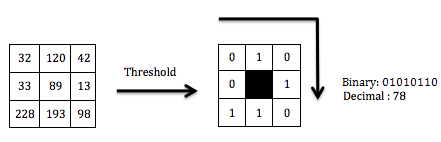
\includegraphics[scale=0.5]{figures/lbp_basic_operator} 
\newline
\caption{Basic LBP operator}
\label{lbp_basic_operator}
\end{center} 
\end{figure}

\noindent Figure~\ref{lbp_basic_operator_example} shows an example of the LBP operator applied on a facial image from the JAFFE database \cite{LIU11}.
\newline

\begin{figure}[!h]
\begin{center}
\noindent 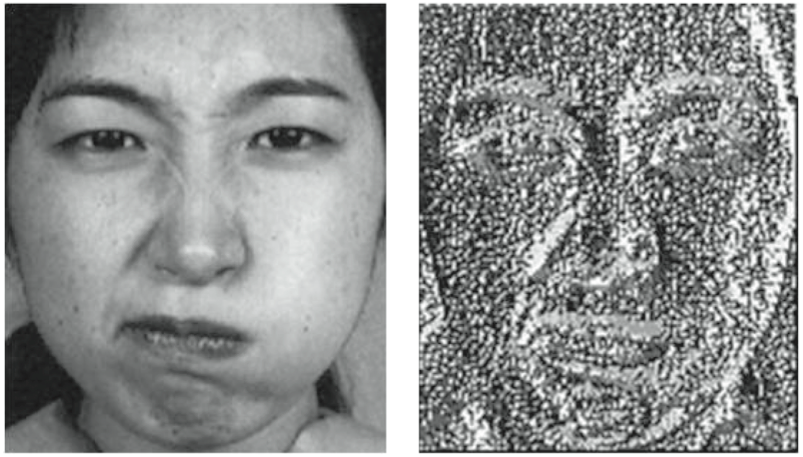
\includegraphics[scale=0.4]{figures/lbp_basic_operator_example} 
\newline
\caption{Example of the LBP operator applied on a image from the JAFFE database}
\label{lbp_basic_operator_example}
\end{center} 
\end{figure}

\phantomsection
\section{Improvements}

\phantomsection
\subsection{Circular LBP}

\vspace{\baselineskip}
\noindent In order to be able to use the LBP operator at different scales, a new form of the operator has been introduced. This new form is the circular LBP operator. This way, the operator can be extended to other neighbourhoods than only eight pixels. \cite{GAN08}.
\newline

\noindent This operator still compares the intensity value of the central pixel with its neighbors, but neighbors pixels are now calculated on a circle as follows \cite{GAN08}:

\begin{itemize}
  \item P represents the number of sampling points (neighbor pixels)
  \item C represents the central pixel with coordinates $ (x_c,y_c) $
  \item R represents the distance between each neighbor pixel and the central one
\end{itemize}

\noindent Coordinates of the p$^{th}$ neighbor pixel are calculated with the following formulas \cite{JUL07}:
\newline

\begin{equation}
   x = x_c + R\cos(2\pi n/P)
\end{equation}

\begin{equation}
   y = y_c + R\sin(2\pi n/P)
\end{equation}

\vspace{\baselineskip}
\noindent Figure~\ref{lbp_circular_operator} shows the circular LBP operator with different numbers of neighbor pixels P and with various radius sizes \cite{JUL07}. For the circular LBP operator, the following notation is used: $ (P,R) $ and for a pixel p, the following notation is used: $ LBP_{P,R}(p) $ \cite{GAN08}.
\newline

\begin{figure}[!h]
\begin{center}
\noindent 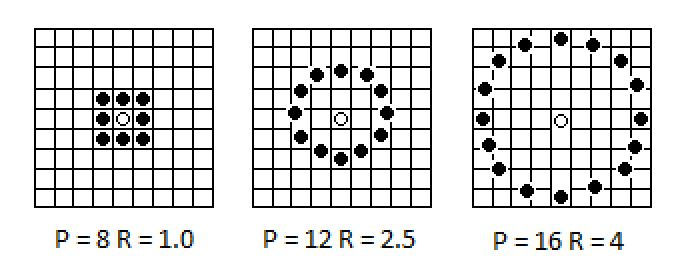
\includegraphics[scale=0.5]{figures/lbp_circular_operator} 
\newline
\caption{Circular LBP operator with different radius sizes R and different number of neighbor pixels P}
\label{lbp_circular_operator}
\end{center} 
\end{figure}

\noindent Most of the time, when a circular LBP operator is used, coordinates of the neighbor pixels (calculated with the formulas given above) may not land exactly on a pixel. In this case, using a bilinear interpolation of neighbor pixels intensity values is recommended. For example, the circular operator with $ P = 8 $ and $ R = 1.0 $ is similar to the basic LBP operator; the only difference being during the calculation, if neighbor pixels do not land exactly onto single pixels, these pixels have to be interpolated first \cite{GAN08}.
\newline

\noindent The LBP operation outputs a texture, which formula is \cite{GAN08}:
\newline

\begin{equation}
   T = t(I_C, I_0, I_1, ..., I_{P-1})
\end{equation}

\vspace{\baselineskip}
\noindent With $ I_C $, the intensity value of central pixel C, $ I_p $ for $ p = 0, 1, ..., P-1 $, the intensity values of the P neighbor pixels, and $ T $, the texture in the local neighborhood of $ C $ \cite{GAN08}.
\newline

\noindent This texture can also be calculated in an other way. The central pixel intensity value can be substracted from the computed neighbourhood values. Output texture $ T $ becomes the combination of differences between intensity values of the neighbor pixels and central pixel, and of the intensity value of the central pixel $ I_C $, resulting in the following formula \cite{GAN08}:
\newline

\begin{equation}
   T = t(I_C, I_0 - I_C, I_1 - I_C, ..., I_{P-1} - I_C)
\end{equation}

\vspace{\baselineskip}
\noindent Based on the work of Ojala et al. \cite{OJA96}, $ t(I_C) $ describes the overall luminance of an image, which is not related to the local texture of the image. Consequently, relevant information for texture analysis are not provided by this value. It can then be discarded without affecting the texture description \cite{GAN08}:
\newline

\begin{equation}
   T = t(I_0 - I_C, I_1 - I_C, ..., I_{P-1} - I_C)
\end{equation}

\vspace{\baselineskip}
\noindent The above formula makes the texture description invariant against shifts in intensity values. t however does not make it invariant against scaling of intensity values. To obtain a texture description invariant to these scalings, only the signs of the differences are taken into account, and not the difference in itself. The new formula is as follows \cite{GAN08}:
\newline

\begin{equation}
   T = t(s(I_0 - I_C), s(I_1 - I_C), ..., s(I_{P-1} - I_C))
\end{equation}

\noindent where,
\newline

\begin{equation}
s(x) = \left\{
    \begin{array}{ll}
        1 & \mbox{if } x\geq0 \\
        0 & \mbox{if } x < 0
    \end{array}
\right.
\end{equation}

\vspace{\baselineskip}
\noindent For the pixels with an intensity value superior or equal to the one of the central pixel, the sign assigned would be 1. For the pixels with an intensity value inferior to $I_C$it  would be 0 \cite{GAN08}.
\newline

\noindent The last step is to assign a binomial weight to each sign, for the LBP operation. These weights are summed, producing an imporved LBP code for central pixel $ C $ with coordinates $ (x_C,y_C) $ \cite{GAN08}:
\newline

\begin{equation}
   LBP_{P,R}(x_C,y_C) = \sum_{p = 0}^{P-1} s(I_p - I_C)2^p
\end{equation}

\vspace{\baselineskip}
\noindent The use of the formula above to calculate LBP still outputs a large number of patterns, which does not help reducing the data size. An other improvement to the LBP operator, called uniform LBP, can then be used to efficiently reduce the data size. This kind of LBP will be explained in the subsection below.
\newline

\phantomsection
\subsection{Uniform LBP}

\vspace{\baselineskip}
\noindent A Local Binary Pattern can be called uniform only if it contains 2 or less bitwise transitions. A bitwise transition is a transition from 0 to 1 or from 1 to 0 \cite{GAN08}. 
\newline

\noindent In fact, there can be only 2 or 0 bitwise transitions for a uniform LBP. Indeed, the neighbourhood is circular so there cannot be 1-bitwise transition in the pattern. Indeed, if there is a bitwise transition in the neighbourhood, i.e from 1 to 0, it means that there will be another bitwise transition from 0 to 1 further in the circular pattern \cite{GAN08}.
\newline

\noindent If a pattern contains 0 bitwise transitions, it means that it is composed only of 0s or of 1s \cite{GAN08}.
\newline

\noindent For a uniform LBP with a pattern-length of 8 bits (i.e 8 neighbours), containing 2 bitwise transitions, with P neighbor pixels, there are $ P(P - 1) $ possible combinations. So there are $ 8(8 - 1) + 2 =58 $ possible patterns ("$ + 2 $" is for the 2 patterns with 0 bitwise transitions. The uniform LBP has the following notation: \[ LBP_{P,R}^{u^2} \] with P numbers of neighbouring pixels and radius size R \cite{GAN08}.
\newline

\noindent There are 2 main advantages coming along with the uniform LBP. The first one is the reduction in range of possible patterns. With the uniform LBP operator, there are 58 possible combinations as seen above, whereas with the basic LBP operator, there are $ 2^8 = 256 $ possible combinations for the same bit-length. The use of uniform LBP then leads to less computation \cite{GAN08}.
\newline

\noindent The second advantage is that, even though there is a reduction of dimensionality, the patterns remain discriminative between various structural features. These structural features detected by the uniform LBP are the spot, the spot/flat, the line end, the edge and the corner, as shown in Figure~\ref{lbp_structural_features}  \cite{GAN08}.
\newline

\begin{figure}[!h]
\begin{center}
\noindent 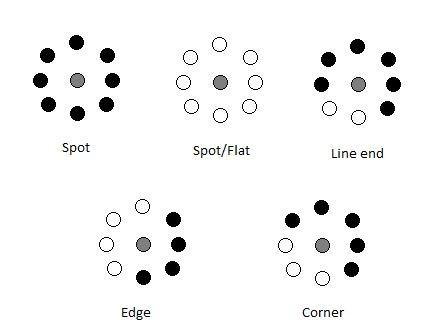
\includegraphics[scale=0.6]{figures/lbp_structural_features} 
\newline
\caption{Patterns that can be detected with uniform LBP}
\label{lbp_structural_features}
\end{center} 
\end{figure}

\phantomsection
\section{Facial Expression Recognition based on LBP}

\vspace{\baselineskip}
\noindent The LBP operator can be used to extract features for a facial expression recognition system. The main idea is to obtain a set of features vectors from the train data, using LBP. After training the classifiers with these feature vectors, test data will then undergo the same LBP feature extraction before classification. 
\newline

\phantomsection
\section{Histogram computing}

\vspace{\baselineskip}
\noindent To obtain these features vectors mentioned above, pixel values obtained with the LBP operator are concatenated into an histogram, which will give feature vectors.
\newline

\noindent To compute this histogram, the face has to be partitioned into regions first. Most of the time, it is partitioned as following: 42 regions, 7 rows and 6 columns. It matches parts of the face yielding important features for emotion recognition. Face dimensions for all tested images should be kept constant. Then for all pixels of the face, their LBP value is computed using $ LBP_{8,2}^{u^2} $. Then, resulting values are gathered region-wise into different bins. For example, the LBP operator with $ P = 8 $ and $ R = 1.0 $ outputs a histogram with 59 bins: 56 bins for uniform LBP with 2 bitwise transitions, 2 bins for  uniform LBP with 0 bitwise transition and the remaining bin for non-uniform patterns). All these bins are concatenated column-wise; as it can be seen in Figure~\ref{lbp_histogram}. The final vector obtained with this histogram is a vector of $ 42\times59 = 2478 $ rows, the histogram being computed for each region partitioned on the sample image \cite{GAN08}.
\newline

\begin{figure}[!h]
\begin{center}
\noindent 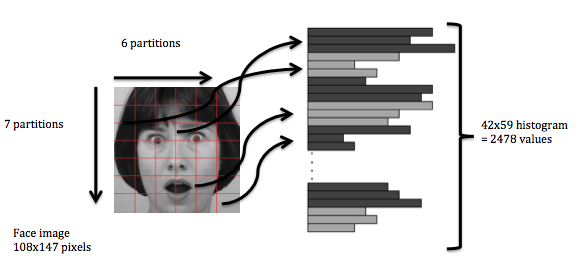
\includegraphics[scale=0.4]{figures/lbp_histogram} 
\newline
\caption{Example of a vector based on histogram computing}
\label{lbp_histogram}
\end{center} 
\end{figure}

\noindent The regions obtained when the sample image is partitioned do not have the same contribution to the expressed emotion. For example, eyes bring more information about an emotion than cheeks. For each region, a weight is then assigned as in Figure~\ref{lbp_region_weight} \cite{GAN08}. Thus, the histogram of each region is multiplied with a corresponding weight.
\newline

\begin{figure}[!h]
\begin{center}
\noindent 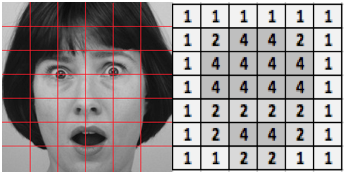
\includegraphics[scale=0.4]{figures/lbp_region_weight} 
\newline
\caption{Weight assignment for each region}
\label{lbp_region_weight}
\end{center} 
\end{figure}
\newpage
